\documentclass{beamer}
\usepackage{textcomp} %textrightarrow
\usepackage{listings}
\usepackage{graphicx}
\usetheme{Boadilla}
\title{Relazione lavoro svolto}
\author{Pietro Ghiglio}

\lstset{ 
  basicstyle=\footnotesize,        
  captionpos=none,                    
  commentstyle=\color{green},    % comment style
  extendedchars=true,              % lets you use non-ASCII characters; for 8-bits encodings only, does not work with UTF-8
  frame=single,	                   % adds a frame around the code
  keywordstyle=\color{blue},       % keyword style
  language=C,                 % the language of the code
  numbers=left,                    
  numbersep=5pt,                   
  numberstyle=\tiny\color{gray}, 
  rulecolor=\color{black},         
  stepnumber=1,                    
  tabsize=2,	                                 
}

\AtBeginSection[]
{
  \begin{frame}
    \frametitle{Table of Contents}
    \tableofcontents[currentsection]
  \end{frame}
}

\begin{document}
\titlepage

\begin{frame}
\frametitle{Table of Contents}
\tableofcontents
\end{frame}


\section{Replaced By Graph}

\begin{frame}
\frametitle{Prima di TailCallElim}
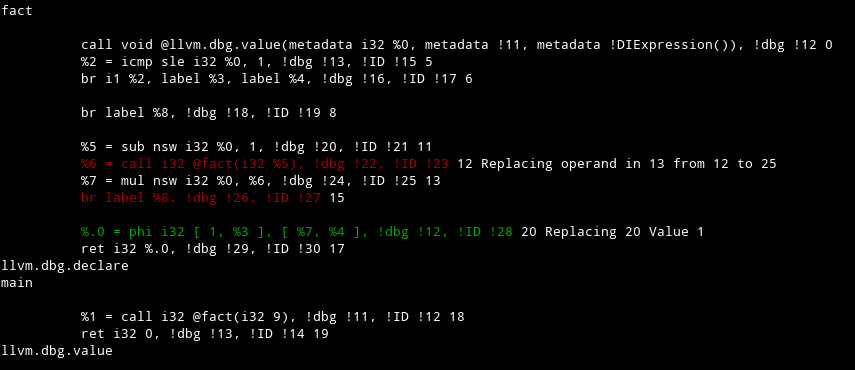
\includegraphics[scale=0.4]{fact_old.png}
\end{frame}

\begin{frame}
\frametitle{Dopo TailCallElim}
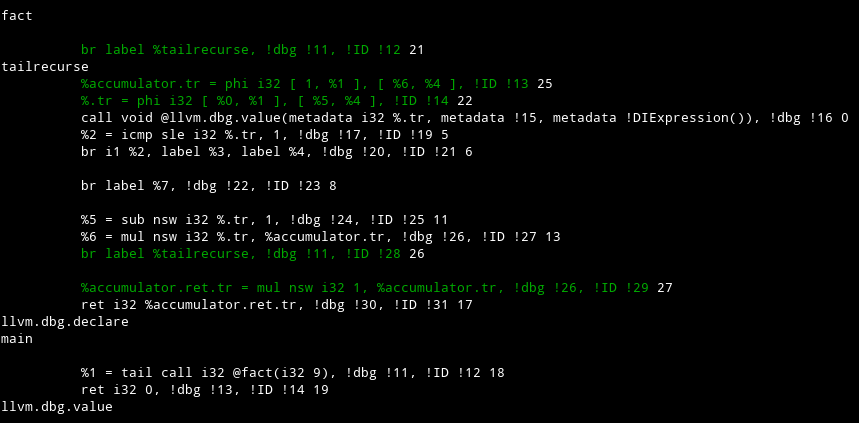
\includegraphics[scale=0.5]{fact.png}
\end{frame}

\begin{frame}
\frametitle{Cosa fare con nuove istruzioni?}
\begin{itemize}
\item Sapere che una nuova istruzione è stata creata non basta per attribuire (automaticamente) info di debug mancanti.
\item Guardare a quali istruzioni vengono sostituite da quelle appena aggiunte.
\item Relazione "Replaced By" tra istruzioni, rappresentata da un grafo.
\end{itemize}
\lstinputlisting[language=C]{node.c}
\end{frame}

\begin{frame}
\frametitle{Propagare Source Locations}
\lstinputlisting[language=C]{prop.c}
\end{frame}

\section{Inlining}

\begin{frame}
\frametitle{Pre Inlining}
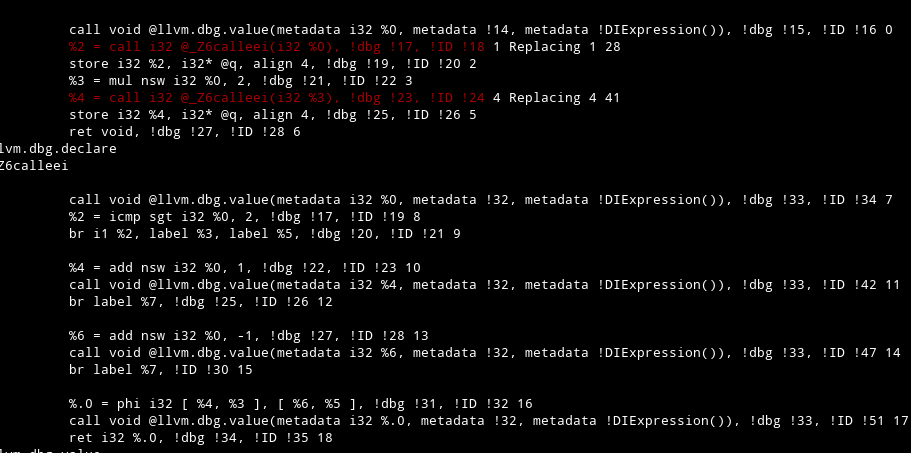
\includegraphics[scale=0.35]{pre_inline.png}
\end{frame}

\begin{frame}
\frametitle{Post Inlining}
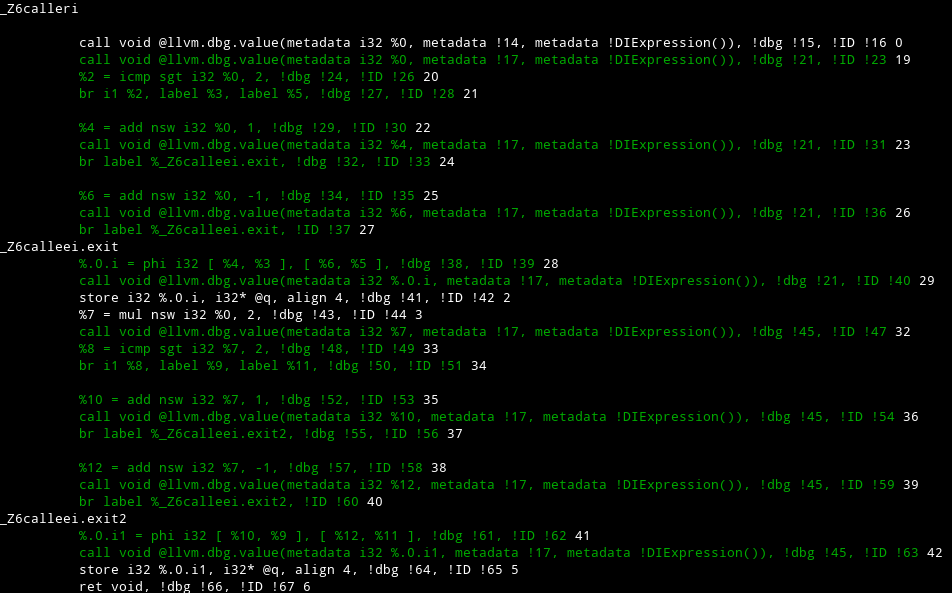
\includegraphics[scale=0.35]{post_inline.png}
\end{frame}

\begin{frame}
\frametitle{Osservazioni}
\begin{itemize}
\item La maggior parte delle istruzioni inserite ha info di debug corrette.
\item I due phi-node che sostinuiscono le call hanno info di debug, ma hanno Line e Column a 0.
\item Propagando le location, gli viene assegnata la location delle call.
\end{itemize}
\end{frame}


\section{SimplifyCFG}

\begin{frame}
\frametitle{Pre Simplify}
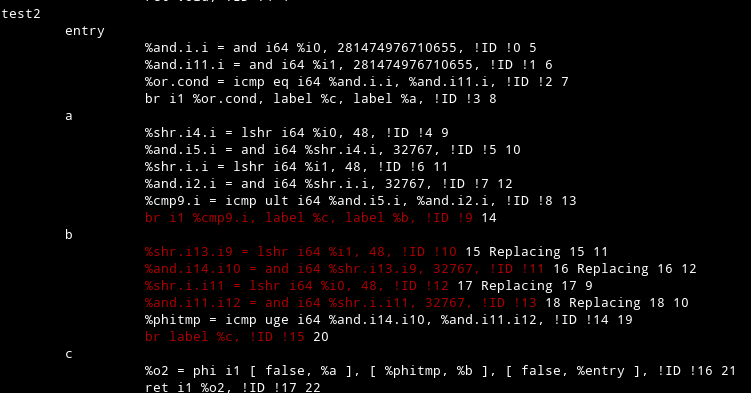
\includegraphics[scale=0.45]{pre_simpl.png}
\end{frame}

\begin{frame}
\frametitle{Post Simplify}
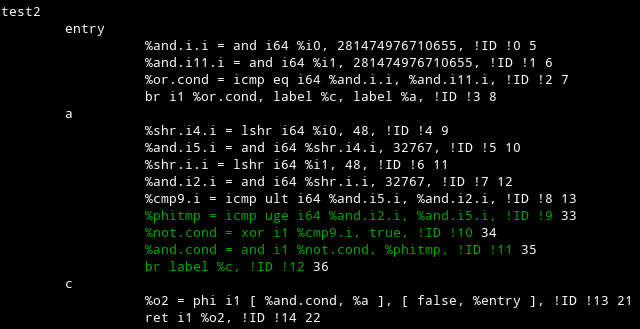
\includegraphics[scale=0.5]{post_simpl.png}
\end{frame}

\begin{frame}
\frametitle{Osservazioni}
\begin{itemize}
\item La istruzioni del basic block b vengono sostituite con istruzioni di a.
\item Propagando le locations, le istruzioni di a avranno due locations (quelle che avevano prima, e quelle di b). \newline
Cosa fare quando si attribuisce il costo energetico?
\end{itemize}
\end{frame}

\section{InstCombine}

\begin{frame}
\frametitle{InstCombine}
Pre: \newline
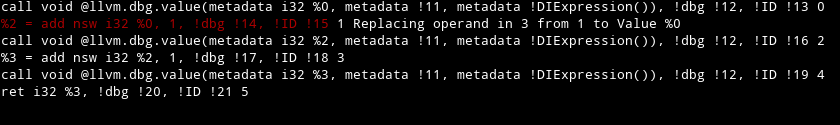
\includegraphics[scale=0.35]{pre_icomb.png}
\newline
Post: \newline
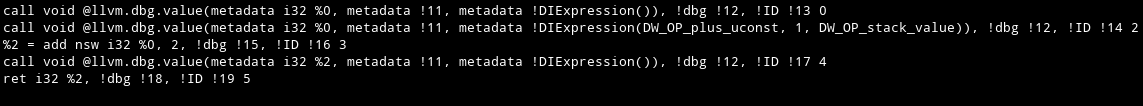
\includegraphics[scale=0.35]{post_icomb.png}
\end{frame}

\begin{frame}
\frametitle{Osservazioni}
\begin{itemize}
\item Per via dell'implementazione della trasformazione, dal log non si evince chiaramente che l'istruzione 3 diventa il merge di 1 e 3.
\item Altri problemi: istruzioni senza usi (store, branch), replace con un value che non è un'istruzione.
\end{itemize}

\end{frame}







\end{document}